\section{Time Escape algoritmy}\label{sec:tea}

Pokud se čtenář dostal až do této části, mohl si všimnout, že jednu kategorii fraktálů jsme zatím zcela vynechali. Přitom právě ta je z velké části zodpovědná za popularitu, které se těší toto odvětví matematiky, zejména \emph{Mandelbrotova množina}\index{Mandebrotova množina}\index{množina!Mandebrotova} (viz obrázek \ref{fig:mandebrotova-mnozina}) pojmenovaná po samotném zakladateli fraktální geometrie.
\begin{figure}[h]
    \centering
    
\includegraphics[width=\textwidth]{ch01-mandelbrotova-mnozina.jpg}
    \caption[Mandebrotova množina]{Mandebrotova množina (Převzato z Wikipedia Commons)\footnotemark}
    \label{fig:mandebrotova-mnozina}
\end{figure}
Tím spíš s faktem, že její definice není v konečném důsledku nikterak složitá\footnotetext{Dostupné z \url{https://en.wikipedia.org/wiki/Mandelbrot\_set\#/media/File:Mandel\_zoom\_00\_mandelbrot\_set.jpg}}.

S pravděpodobně nejznámějším fraktálem však souvisí dvojice širších termínů, se kterým začneme, a jsou jimi tzv. \emph{Juliovy množiny}\index{Fatouova množina}\index{množina!Fatouova} a \emph{Fatouovy množiny}\index{Fatouova množina}\index{množina!Fatouova} pojmenované po francouzských matematicích \name{Gastonovi Juliovi} (1893--1978) a \name{Pierre Fatouovi} (1878--1929). Pro jejich studium se však budeme muset ponořit do světa komplexních čísel.

Lze nejspíše předpokládat, že se čtenář nejspíše s komplexními čísly již setkal. Nebudeme se tedy společně hlouběji zabývat naprostými základy. Pouze si stručně připomeňme značení.
\begin{itemize}
    \item \emph{Komplexním číslem}\index{komplexní číslo} rozumíme číslo $z=a+b\imag$, kde $a,b\in\R$ a $\imag^2=-1$. Množinu komplexních čísel, jak už je zvykem, budeme značit $\C$.
    \item \emph{Komplexně sdruženým číslem}\index{Komplexně sdružerné číslo} k číslu $z=a+b\imag$ rozumíme číslo
    \[\cconjugate{z}=a-b\imag.\]
    \item \emph{Absolutní hodnotou komplexního čísla} $z=a+b\imag$ rozumíme vzdálenost od počátku, tj. budeme-li uvažovat metrický prostor $(\C,\varrho)$, pak
    \[|z|=\varrho(z,0).\]
    Nejčastěji však budeme uvažovat eukleidovskou metriku $\varrho_e$, tedy
    \[|z|=\sqrt{a^2+b^2}.\]
\end{itemize}
V této sekci budeme především pracovat s komplexními polynomiálními funkcemi $\mapping{f}{\C}{\C}$, tzn. funkcemi ve tvaru
\[f(z)=\sum_{i=1}^{n}a_iz^i=a_nz^n+a_{n-1}z^{n-1}+\dots+a_1z+a_0.\]
Brzy uvidíme jejich důležitou roli.

\subsection{Juliovy a Fatouovy množiny}\label{subsec:juliovy-fatouovy-mnoziny}

Jak zde již bylo řečeno, esencí této kapitoly bude práce s tzv. \emph{Juliovými a Fatouovými množinami}\index{Juliova množina}\index{množina!Juliova}\index{Fatouova množina}\index{množina!Fatouova}. Většinový výklad v této části je převzat z knihy \cite[str. 235]{Falconer1989}, avšak řadu věcí si opět dovolíme přeskočit. Dále ještě připomeňme značení, které jsme zavedli již v části \ref{subsec:hausdorffuv-mp-kontrakce} věnující se IFS na Hausdorffově metrickém prostoru, týkající se skládání funkcí. Obecně $n$-tou iteraci funkce $\mapping{f}{\C}{\C}$ budeme značit
\[f^{\circ n}(z)=(f\circ f^{\circ(n-1)})(z)=f(f^{\circ n}(z))\]
kde $z\in\C$.
\begin{definition}[Juliova a Fatouova množina]\label{juliova-fatouova-mnozina}
    Mějme polynomiálními funkci $\mapping{f}{\C}{\C}$. Pak definujeme
    \begin{enumerate}[label=(\alph*)]
        \item \emph{vyplněnou Juliovu množinu}\index{množina!vyplněná Juliova}\index{vyplněná Juliova množina} polynomiální funkce $f$
        \[\filledinjulia(f)=\set{z\in\C\mid f^{\circ n}(z)\notto\infty}.\]
        \item \emph{Juliovu množinu}\index{Juliova množina}\index{množina!Juliova} polynomiální funkce $f$
        \[\julia(f)=\boundary{\filledinjulia(f)}.\]
        \item \emph{Fatouovu množinu}\index{Fatouova množina}\index{množina!Fatouova} polynomiální funkce $f$
        \[\fatou(f)=\C\setminus\julia(f).\]
    \end{enumerate}
\end{definition}
Co nám definice \ref{juliova-fatouova-mnozina} vlastně říká? U pevně zadané funkce $f(z)=\sum_{i=1}^{n}a_iz^i$ pro zadaný bod $z\in\C$ zkoumáme, zda je posloupnost\footnote{Poznamenejme, že limitu posloupnosti komplexní čísel zde chápeme (stejně jako v ostatních případech) jako limitu posloupnosti v metrickém prostoru, jmenovitě $(\C,\varrho_e)$.} jejích postupných iterací $\set{f^{\circ n}(z)}_{n=1}^\infty$ omezená. Později uvidíme, že Juliova množina má v typickém případě charakter fraktálu.
\begin{example}
    \begin{itemize}
        \item Uvažujme identitu $f(z)=z^k$. Pak pro její $n$-tou iteraci platí $f^{\circ n}(z)=z^{k^n}$. Tedy
        \[\filledinjulia(f)=\set{z\in\C\mid |z|<1},\]
        resp.
        \[\julia(f)=\set{z\in\C\mid|z|=1}.\]
        Juliova množina funkce $f$ tvoříjednotkovou kružnici umístěnou v počátku, resp. Juliova množina $J(f)$ tvoří jednotkový kruh.
        \item Pro $f(z)=z^2+c$, kde $c\in\C$ je varianta množiny $K(f)$ znázorněna na obrázku \ref{subfig:vyplnena-juliova-mnozina-1}.
        \item Ještě jiný příklad pro složitější polynom $f(z)=z^3-z^2$ lze vidět na obrázku \ref{subfig:vyplnena-juliova-mnozina-2}.
        \item Pro příklady Juliových množin zadaných polynomů viz obrázky \ref{subfig:juliova-mnozina-1} a \ref{subfig:juliova-mnozina-2}.
    \end{itemize}
\end{example}
\begin{figure}[h]
    \centering
    \begin{subfigure}{0.45\textwidth}
        \centering
        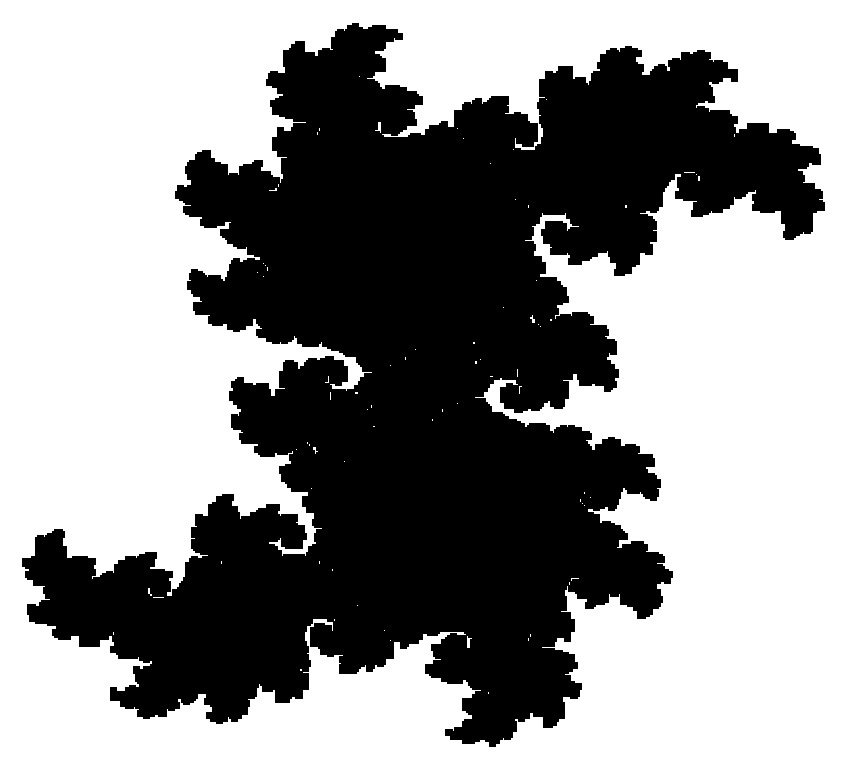
\includegraphics[width=\textwidth]{julia-set-1.pdf}
        \caption{$f(z)=z^2+0.35 + 0.35\imag$}
        \label{subfig:vyplnena-juliova-mnozina-1}
    \end{subfigure}
    \qquad
    \begin{subfigure}{0.45\textwidth}
        \centering
        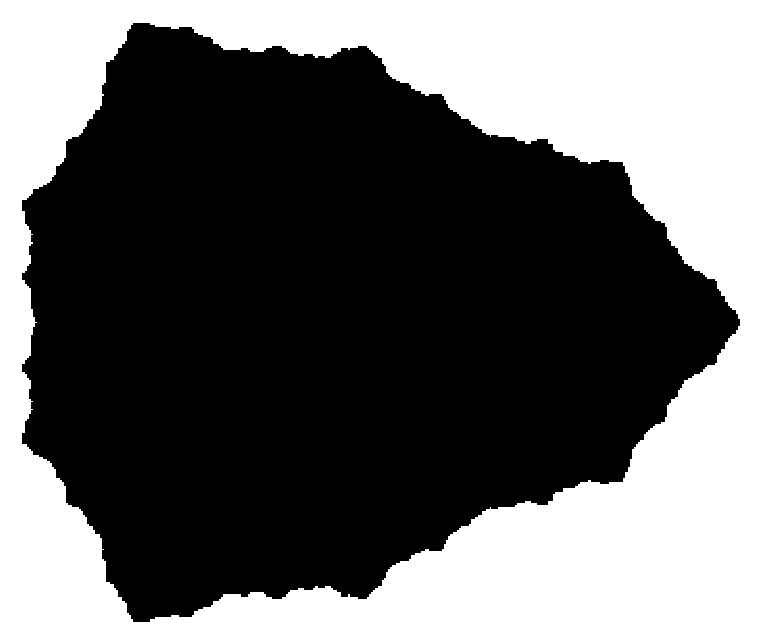
\includegraphics[width=\textwidth]{julia-set-2.pdf}
        \caption{$f(z)=z^3-z^2$}
        \label{subfig:vyplnena-juliova-mnozina-2}
    \end{subfigure}
    \caption{Příklady aproximace $\filledinjulia(f)$}
    \label{fig:priklady-vyplnenych-juliovych-mnozin}
\end{figure}
\begin{figure}[h]
    \centering
    \begin{subfigure}{0.45\textwidth}
        \centering
        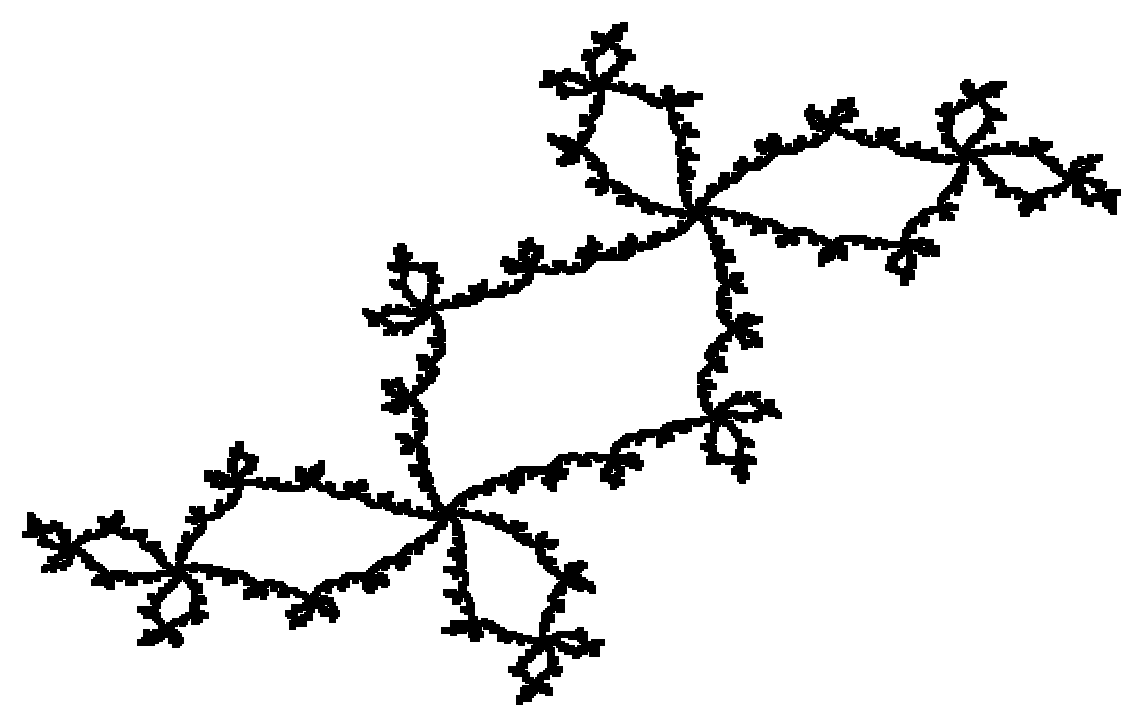
\includegraphics[width=\textwidth]{julia-set-1-boundary.pdf}
        \caption{$f(z)=z^2 + 0{,}7885\cdot e^{\imag\cdot9\pi/16}$}
        \label{subfig:juliova-mnozina-1}
    \end{subfigure}
    \qquad
    \begin{subfigure}{0.45\textwidth}
        \centering
        
\includegraphics[width=\textwidth]{julia-set-2-boundary.pdf}
        \caption{$f(z)=z^2 - 0{,}8 + 0{,}156\imag$}
        \label{subfig:juliova-mnozina-2}
    \end{subfigure}
    \caption{Příklady aproximace $\julia(f)$}
    \label{fig:priklady-juliovych-mnozin}
\end{figure}
Jak jsme již konstatovali, u polynomiální funkce $f$ nás pro zadaný bod $z\in\C$ pouze zajímá, zda posloupnost postupných iterací je omezená. To znamená, že moho nastat dva přípustné scénáře: posloupnost iterací je buď \emph{periodická}, nebo \emph{konvergentní}.

V souvislosti se zmíněnými záležitostmi si nyní dokážeme několik základních poznatků. Řadu dalších však z technických důvodů vynecháme, především ty využívající znalostí z komplexní analýzy. Začneme tvrzením, které se nám později bude hodit při generování tohoto typu fraktálů.
\begin{lemma}\label{lem:test-konvergence-komplexniho-polynomu}
    Nechť je dána polynomiální funkce $\mapping{f}{\C}{\C}$ stupně $n\geqslant 2$. Pak platí následující:
    \begin{enumerate}[label=(\roman*)]
        \item Existuje $r\in\R$, takové, že pokud platí $|z|\geqslant r$, pak $|f(z)|\geqslant2|z|$.
        \item Navíc pokud existuje $m\in\N$, takové, že platí-li $|f^{\circ m}(z)|\geqslant r$, pak $f^{\circ k}(z)\to\infty$.
    \end{enumerate} 
\end{lemma}
\begin{proof}
    Nechť je dáno $z\in\C$. Volme $r\in\R$, takové, že je-li splněno $|z|\geqslant r$, pak platí nerovnost $\frac{1}{2}|a_n||z|^n\geqslant 2|z|$ a zároveň
    \[|a_{n-1}||z|^{n-1}+|a_{n-2}||z|^{n-2}+\dots+|a_1||z|+|a_0|\leqslant\frac{1}{2}|a_n||z|^n.\]
    Předpokládejme tedy, že $|z|>r$. Pak z trojúhelníkové nerovnosti plyne
    \begin{align*}
        |f(z)|&=\left|\sum_{i=0}^{n}a_iz^i\right|\geqslant|a_n||z|^n-\sum_{i=0}^{n-1}|a_i||z|^i\geqslant|a_n||z|^n-\frac{1}{2}|a_n||z|^n\\
        &=\frac{1}{2}|a_n||z|^n\geqslant2|z|.
    \end{align*}
    Pokud navíc platí, že existuje $m\in\N$, takové, že $|f^{\circ m}(z)|\geqslant r$, pak indukcí lze odvodit, že pro $m+k$, kde $k\in\N$, platí
    \[|f^{m+k}(z)|\geqslant2^m|f^{\circ k}(z)|\geqslant r,\]
    neboli $f^{\circ k}(z)\to\infty$.
\end{proof}
(Převzato z \cite[str. 237]{Falconer1989}.)

V čem je lemma \ref{lem:test-konvergence-komplexniho-polynomu} užitečné? V podstatě nám říká, že pro test "chování" posloupnosti $\set{f^{\circ k}(z)}_{n=1}^\infty$ stačí kontrolovat, zda absolutní hodnota obrazu v $k$-té iteraci není vyšší, než zvolené $r$. Pokud ano, je již jasné, že posloupnost bude divergovat. Toho využijeme hlavně při generování fraktálů (viz kapitola \ref{chapter:generovani-fraktalu}).
\begin{example}
    Vezměme si funkci $f(z)=z^2+c$, kde $c\in\C$. Podle věty \ref{lem:test-konvergence-komplexniho-polynomu} při volbě vhodného $r\in\R$, konkrétně $|z|>r$ bude platit, že $|z^2+c|\geqslant|z|^2-|c|\geqslant 2|z|$. Tedy řešíme nerovnici
    \[r^2-|c|\geqslant 2r.\]
    Aplikací známého vzorce dostaneme
    \[r\geqslant\frac{-2+2\sqrt{1+|c|}}{2}=-1+\sqrt{1+|c|}.\]
    Je celkem jasné, že záporný kořen zde nemá smysl. Zároveň však potřebujeme zajistit, aby hodnota na levé straně byla kladná:
    \begin{align*}
        r^2-|c|&\geqslant 2r\\
        r^2-2r&\geqslant|c|\geqslant 0\\
        r(r-2)&\geqslant 0
    \end{align*}
    To platí pro $r\in\langle 2,\infty)$. Pro test divergence posloupnosti $\set{f^{\circ k}(z)}_{n=1}^\infty$ stačí kontrolovat, zda obecně v $k$-té iteraci platí, že
    \[|z^2+c|\geqslant r.\]
    Pro funkce tohoto tvaru se často volí právě $r=2$.
\end{example}
O Juliových množinách lze dokázat některé základní vlastnosti.
\begin{theorem}\label{thm:vztah-kf-a-jf}
    Nechť $f$ je komplexní polynomiální funkce. Pak
    \begin{enumerate}[label=(\roman*)]
        \item\label{thm:kompaktnost-kf-jf} $\filledinjulia(f)$ a $\julia(f)$ jsou neprázdné kompaktní množiny,
        \item\label{thm:jf-podmnozina-kf} $\julia(f)\subseteq \filledinjulia(f)$,
        \item\label{thm:vnitrek-jf-neprazdny} $\interior{(\julia(f))}=\emptyset$.
    \end{enumerate}
\end{theorem}
\begin{proof}
    Z lemmatu \ref{lem:test-konvergence-komplexniho-polynomu} víme, že existuje $r\in\R$, takové, že pokud pro nějaké $m\in\N$ platí $|f^{\circ m}(z)|\geqslant r$, pak $f^{\circ k}\to\infty$. Tedy množiny $\filledinjulia(f)$ a $\julia(f)$ jsou obsaženy v kouli o poloměru $r$ umístěné v počátku, tj.
    \[\filledinjulia(f),\julia(f)\subseteq B_r(0).\]
    Volme $z\in\C\setminus\filledinjulia(f)$, tzn. $f^{\circ k}(z)\to\infty$. Tedy nutně existuje $m\in\N$, takové, že $|f^{\circ m}(z)|>r$. Protože však $f$ je spojitá funkce, existuje $\varepsilon>0$, takové, že pro každé $w\in B_\varepsilon(z)\setminus\set{z}$ platí $f^{\circ k}(w)\to\infty$ a tedy $w\in\C\setminus\filledinjulia(f)$. To znamená, že množina $\C\setminus\filledinjulia(f)$ je otevřená, tedy $\filledinjulia(f)$ je uzavřená množina. Podle Heineho-Borelovy věty \ref{thm:heine-borel} jsou tedy $\filledinjulia(f)$ a $\julia(f)$ kompaktní\footnote{Heineho-Borelovu větu jsme sice formulovali pro $\R^n$, avšak $\C\simeq\R^2$.}. Podle základní věty algebry má rovnice $f(z)=z$ alespoň jedno řešení, označme jej $z_0$. Tedy $f^{\circ k}(z_0)=z_0$, kde $k\in\N$, z čehož plyne, že $z_0\in\filledinjulia(f)$, tzn. $\filledinjulia(f)\neq\emptyset$. Tím jsou dokázány body \ref{thm:kompaktnost-kf-jf} a \ref{thm:jf-podmnozina-kf}.
    
    Dále si zvolme $z_1\in\C\setminus\filledinjulia(f)$ a uvažujme funkci $l(\lambda)=\lambda z_0+(1-\lambda)z_1$, kde $0\leqslant\lambda\leqslant 1$. Tedy $l$ představuje spojnici bodů $z_0$ a $z_1$. Položme
    \[\lambda^\prime=\sup\set{\lambda\in\langle0,1\rangle\mid l(\lambda)\in\filledinjulia(f)}.\]
    Tzn. musí ležet na její hranici, tedy $l(\lambda^\prime)\in\boundary{\filledinjulia(f)}=\julia(f)$. Z toho plyne, že i $\julia(f)$ je neprázdná množina.

    Poslední bod \ref{thm:vnitrek-jf-neprazdny} dokážeme sporem. Pokud by byla množina $\interior{(\julia(f))}$ neprázdná, pak by existovala neprázdná otevřená množina $U\subseteq\julia(f)\subseteq\filledinjulia(f)$. To by znamenalo, že $U\subseteq\interior{(\filledinjulia(f))}$ a zároveň má $U$ neprázdný průnik s hranicí $\filledinjulia(f)$, což je spor.
\end{proof}
(Převzato z \citep[str. 237]{Falconer1989}.)
\begin{theorem}\label{invariance-jf}
    Je-li $f$ libovolná komplexní polynomiální funkce, pak $\julia(f)$ je invariantní vůči $f$. Tzn.
    \[\julia(f)=f(\julia(f))=f^{-1}(\julia(f)).\]
\end{theorem}
\begin{proof}
    Nechť $z\in\julia(f)$. Z bodu \ref{thm:jf-podmnozina-kf} tvrzení \ref{thm:vztah-kf-a-jf} plyne, že $f^{\circ k}(z)\notto\infty$. Najdeme posloupnost $\set{\omega_n}_{n=1}^\infty$, takovou, že $\omega_n\to z$ a zároveň $f^{\circ k}(\omega_n)\to\infty$ pro všechna $n\in\N$. Ze spojitosti funkce $f$ plyne, že $f(\omega_n)\to f(z)$, přičemž $f^{\circ k}(f(z))=f^{\circ(k+1)}(z)\to\infty$ a $f^{\circ k}(f(\omega_n))=f^{\circ(k+1)}(\omega_n)\to\infty$ pro každé $n\in\N$. Z toho plyne, že $f(z)\in\julia(f)$ a tedy $f(\julia(f))\subseteq\julia(f)$. Dále rovněž máme
    \[\julia(f)\subseteq f^{-1}(f(\julia(f)))\subseteq f^{-1}(\julia(f)).\]

    Druhou inkluzi ukážeme obdobně. Definujme posloupnost $\set{\omega_n}_{n=1}^\infty$ jako výše. Najdeme $z_0$, takové, že $f(z_0)=z\in\julia(f)$. Poté můžeme nalézt posloupnost $\set{v_n}_{n=1}^\infty$, tak, aby platilo $f(v_n)=\omega_n$ pro každé $n\in\N$, tzn.
    \[f(v_n)=\omega_n\to z=f(z_0).\]
    Zároveň však platí $f^{\circ k}(z_0)=f^{\circ(k-1)}(z)\notto\infty$ a $f^{\circ k}(v_n)=f^{\circ(k-1)}(\omega_n)\to\infty$, tedy $z_0\in\julia(f)$. Z toho plyne, že $f^{-1}(\julia(f))\subseteq\julia(f)$, neboli $\julia(f)=f(f^{-1}(\julia(f)))\subseteq f(\julia(f))$.
\end{proof}
\begin{theorem}\label{ekvivalence-jf-a-jfp}
    Nechť $f$ je libovolná polynomiální funkce. Pak $\julia(f)=\julia(f^{\circ p})$ pro libovolné $p\in\N$.
\end{theorem}
\begin{proof}
    Z lemmatu \ref{lem:test-konvergence-komplexniho-polynomu} plyne, že $f^{\circ k}(z)\to\infty$ právě tehdy, když $(f^{\circ p})^{\circ k}(z)=f^{\circ kp}(z)\to\infty$. Tedy $\fatou(f)=\fatou(f^{\circ p})$, z čehož plyne $\julia(f)=\julia(f^{\circ p})$.
\end{proof}
(Převzato z \citep[str. 238]{Falconer1989}.)

Pro základní přehled nám tyto vlastnosti budou stačit. Pro další informace doporučuji se podívat do citované literatury.

Vraťme se na chvíli k obrázkům \ref{fig:priklady-vyplnenych-juliovych-mnozin} a \ref{fig:priklady-juliovych-mnozin}. Vzhledem k rozšířenosti tohoto typu fraktálů (a to mnohdy i mezi širší matematiky zainteresovanou veřejností) si čtenář možná mohl všimnout, že zatímco v těchto případech jsme body náležící příslušné (vyplněné) Juliově množině vybarvili černou barvou, na obrázku \ref{fig:mandebrotova-mnozina} je zbarvení podstatně sofistikovanější\footnote{A leckdo by jej nejspíše shledal i krásnějším.}. Příklady takového způsobu znázornění si lze prohlédnout na obrázcích \ref{subfig:vyplnena-juliova-mnozina-1-obarveno} a \ref{subfig:vyplnena-juliova-mnozina-2-obarveno}. Obrázky jsou opět vygenerovány pomocí přiloženého programu.
\begin{figure}[h]
    \centering
    \begin{subfigure}{0.48\textwidth}
        \centering
        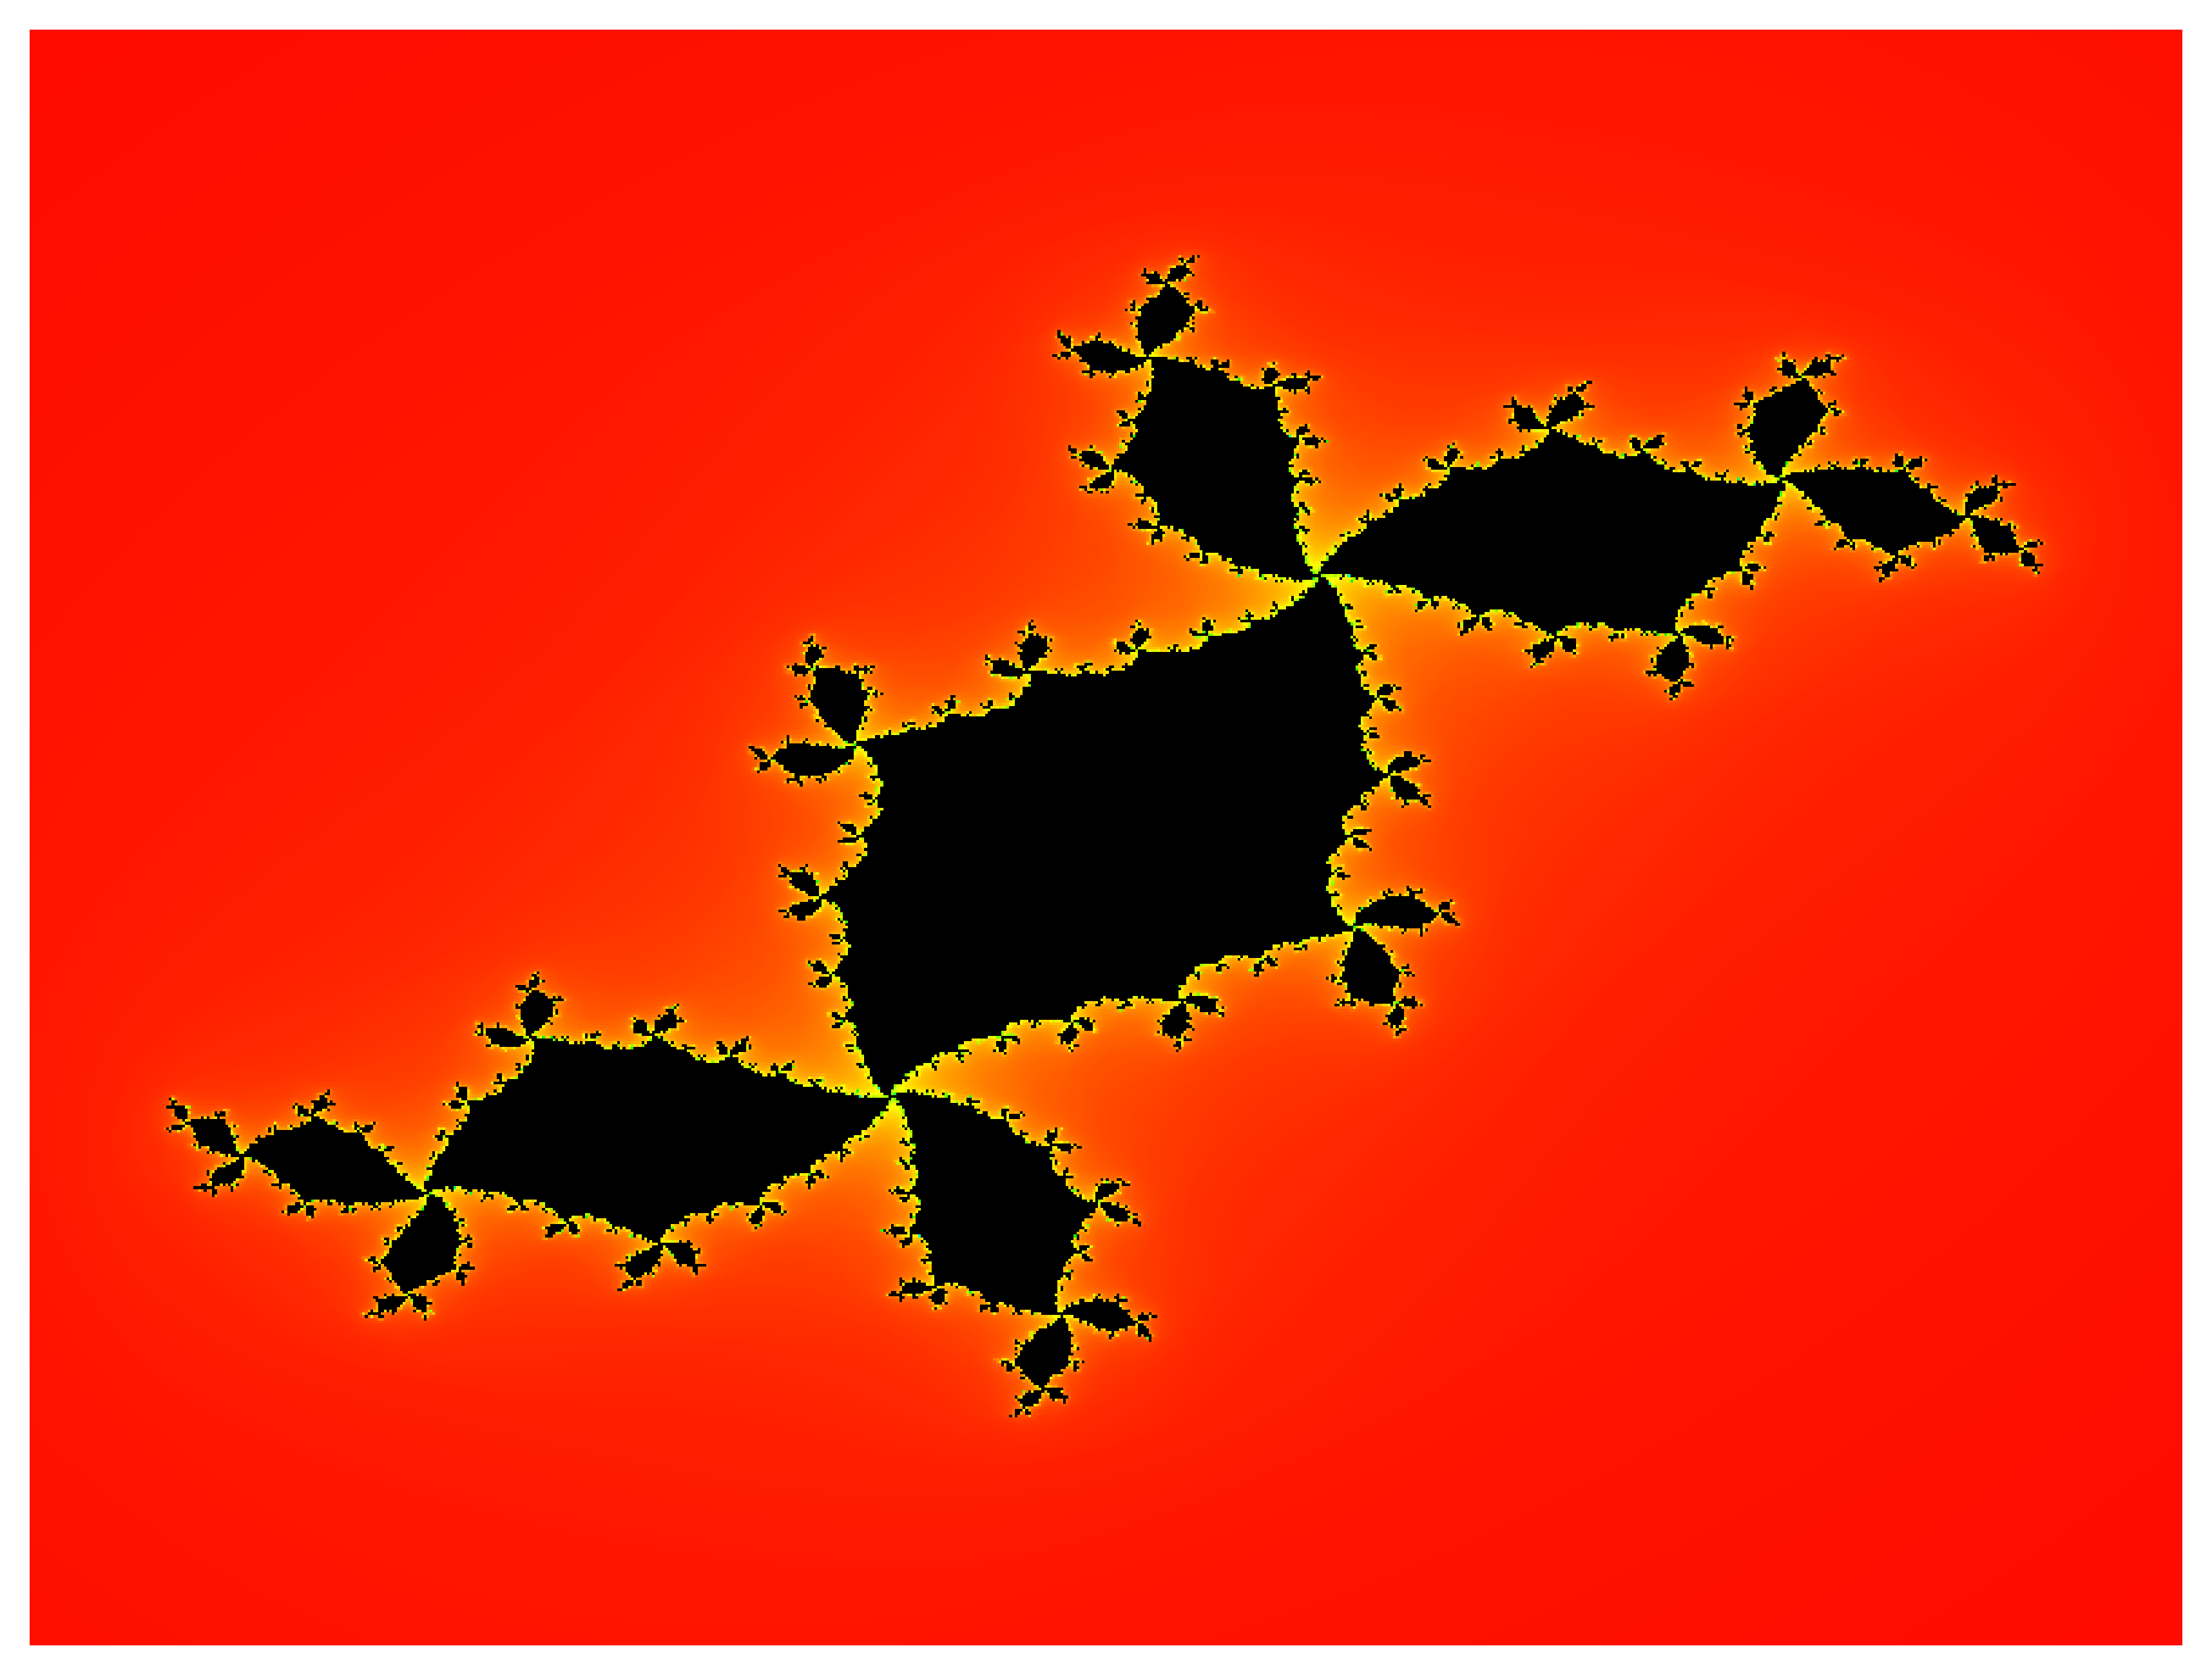
\includegraphics[width=\textwidth]{julia-set-1-colored.png}
        \caption{$f(z)=z^2 + 0{,}7885\cdot e^{\imag\cdot9\pi/16}$}
        \label{subfig:vyplnena-juliova-mnozina-1-obarveno}
    \end{subfigure}
    \quad
    \begin{subfigure}{0.48\textwidth}
        \centering
        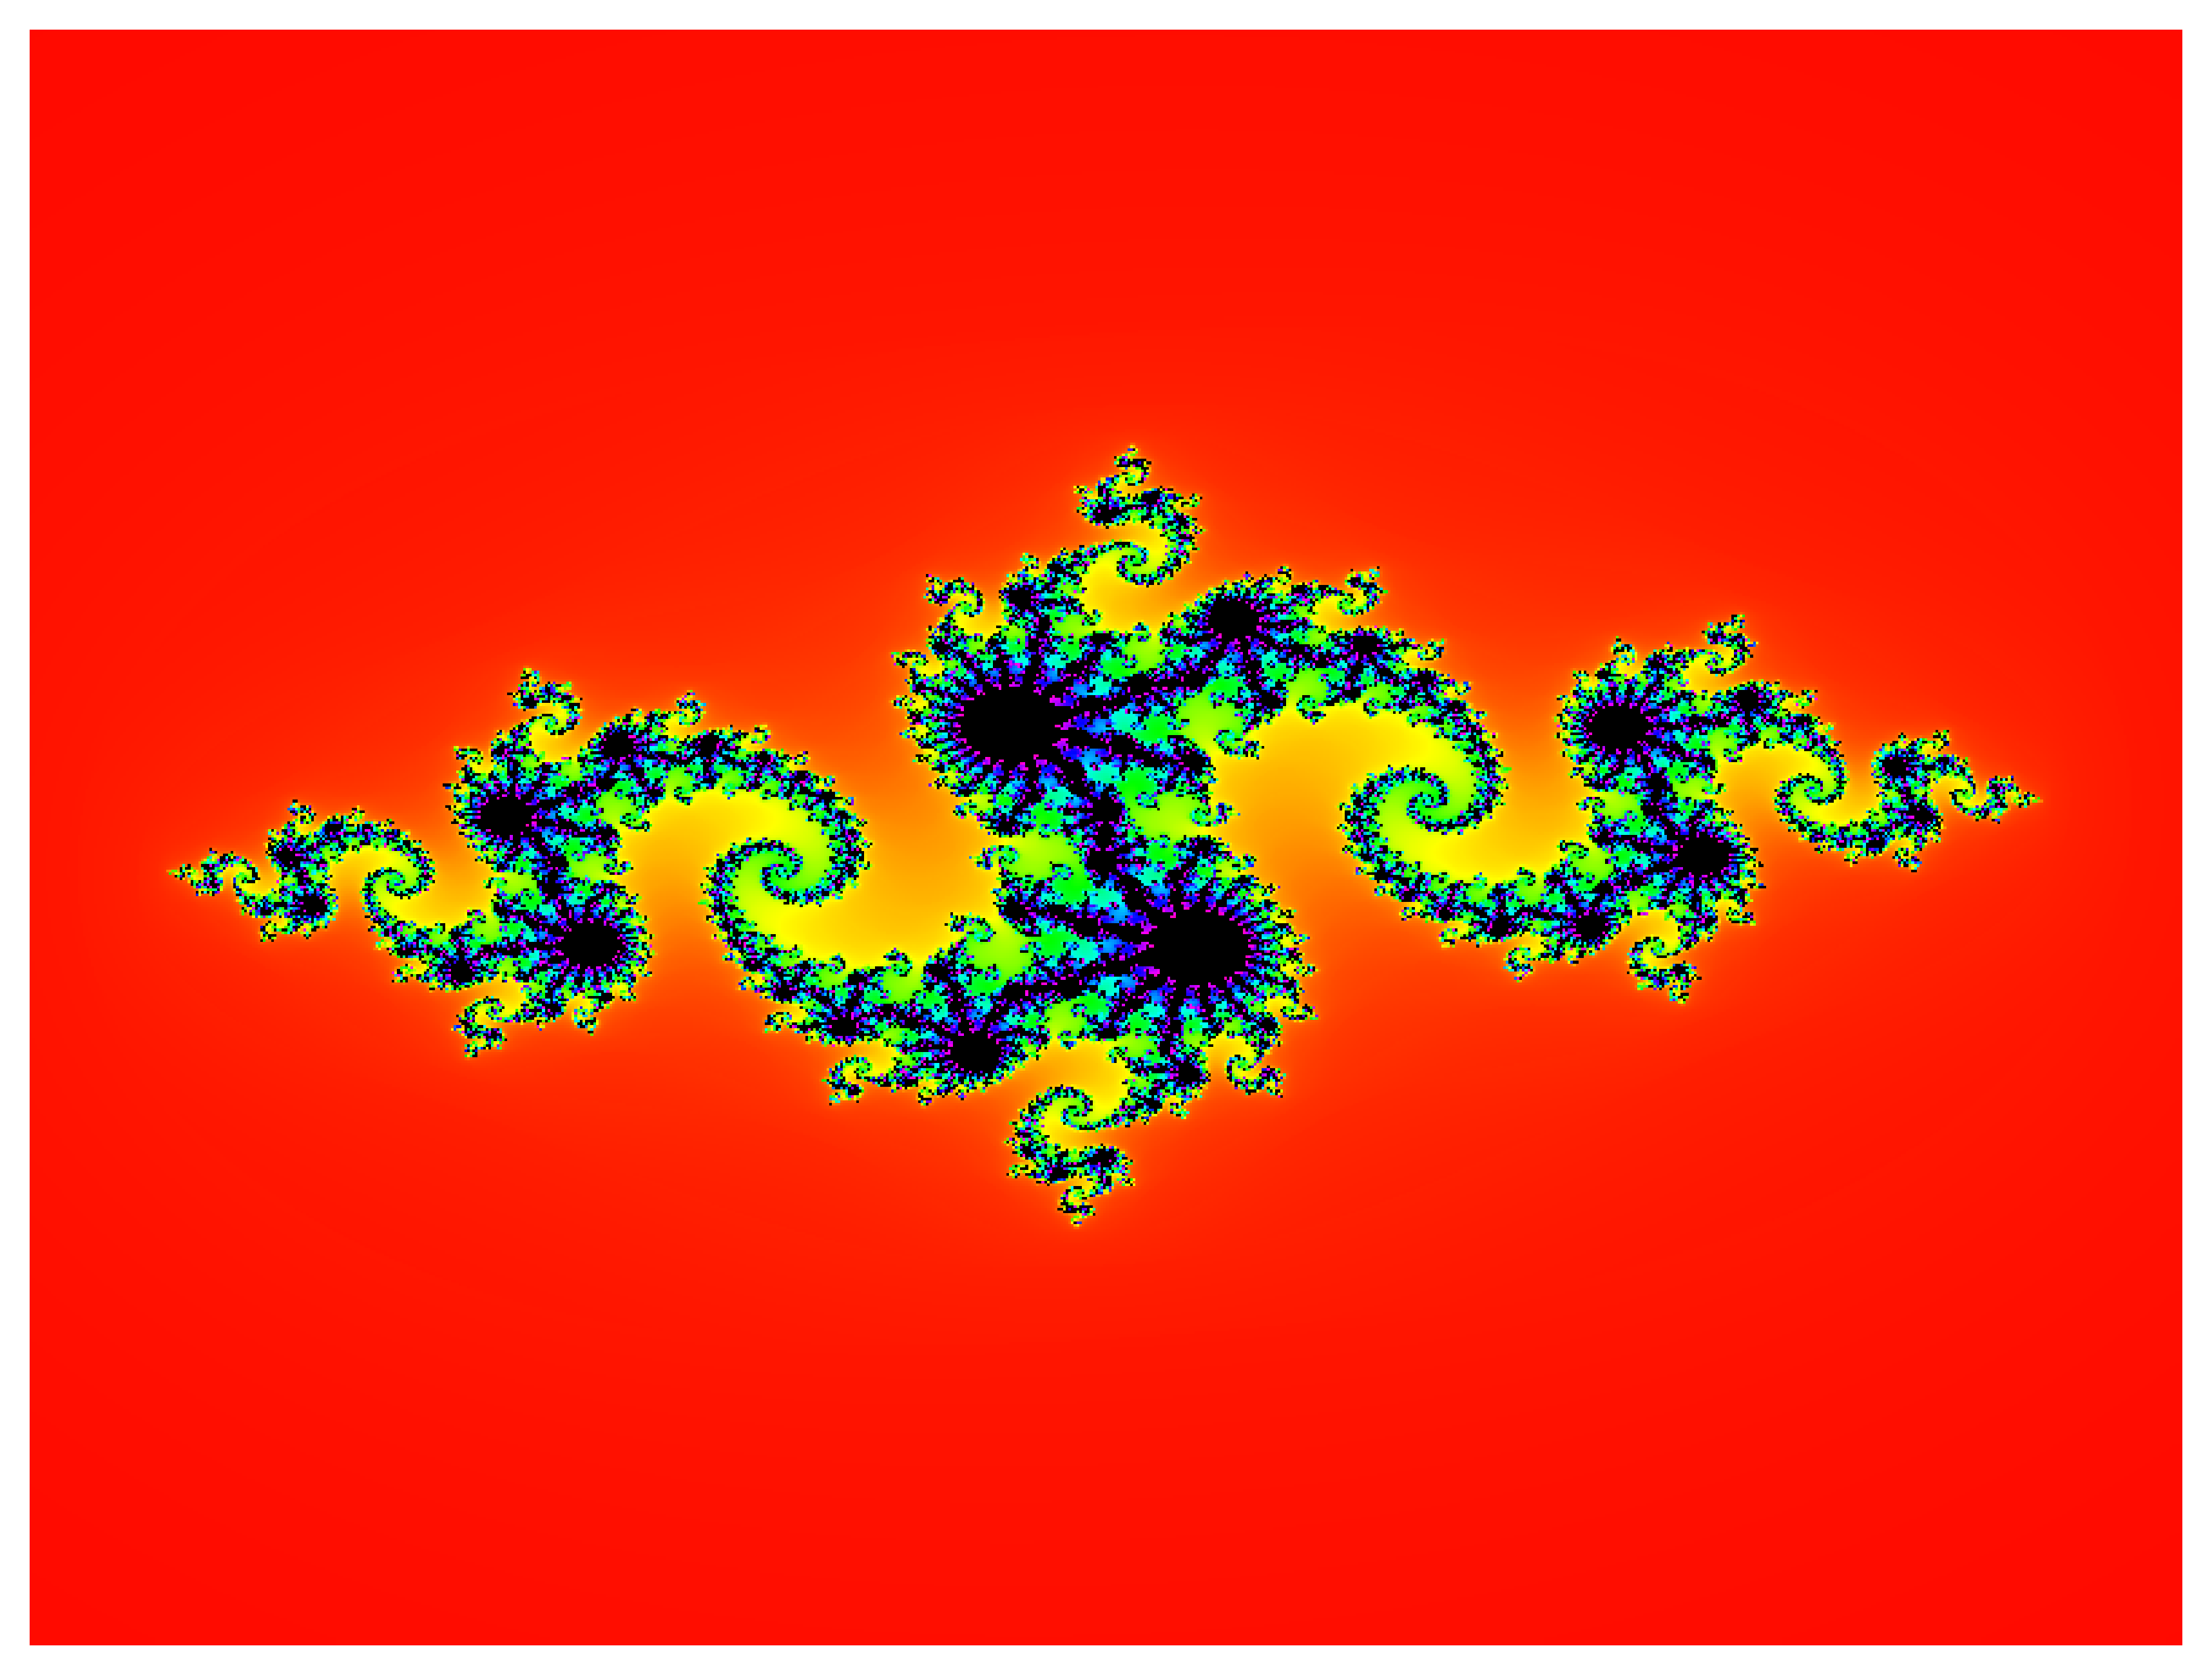
\includegraphics[width=\textwidth]{julia-set-2-colored.png}
        \caption{$f(z)=z^2 - 0{,}8 + 0{,}156\imag$}
        \label{subfig:vyplnena-juliova-mnozina-2-obarveno}
    \end{subfigure}
    \caption{Příklady zbarvení bodů pro různé $\filledinjulia(f)$.}
    \label{fig:priklady-vyplnenych-juliovych-mnozin-obarveno}
\end{figure}
% \begin{figure}[H]
%     \centering
%     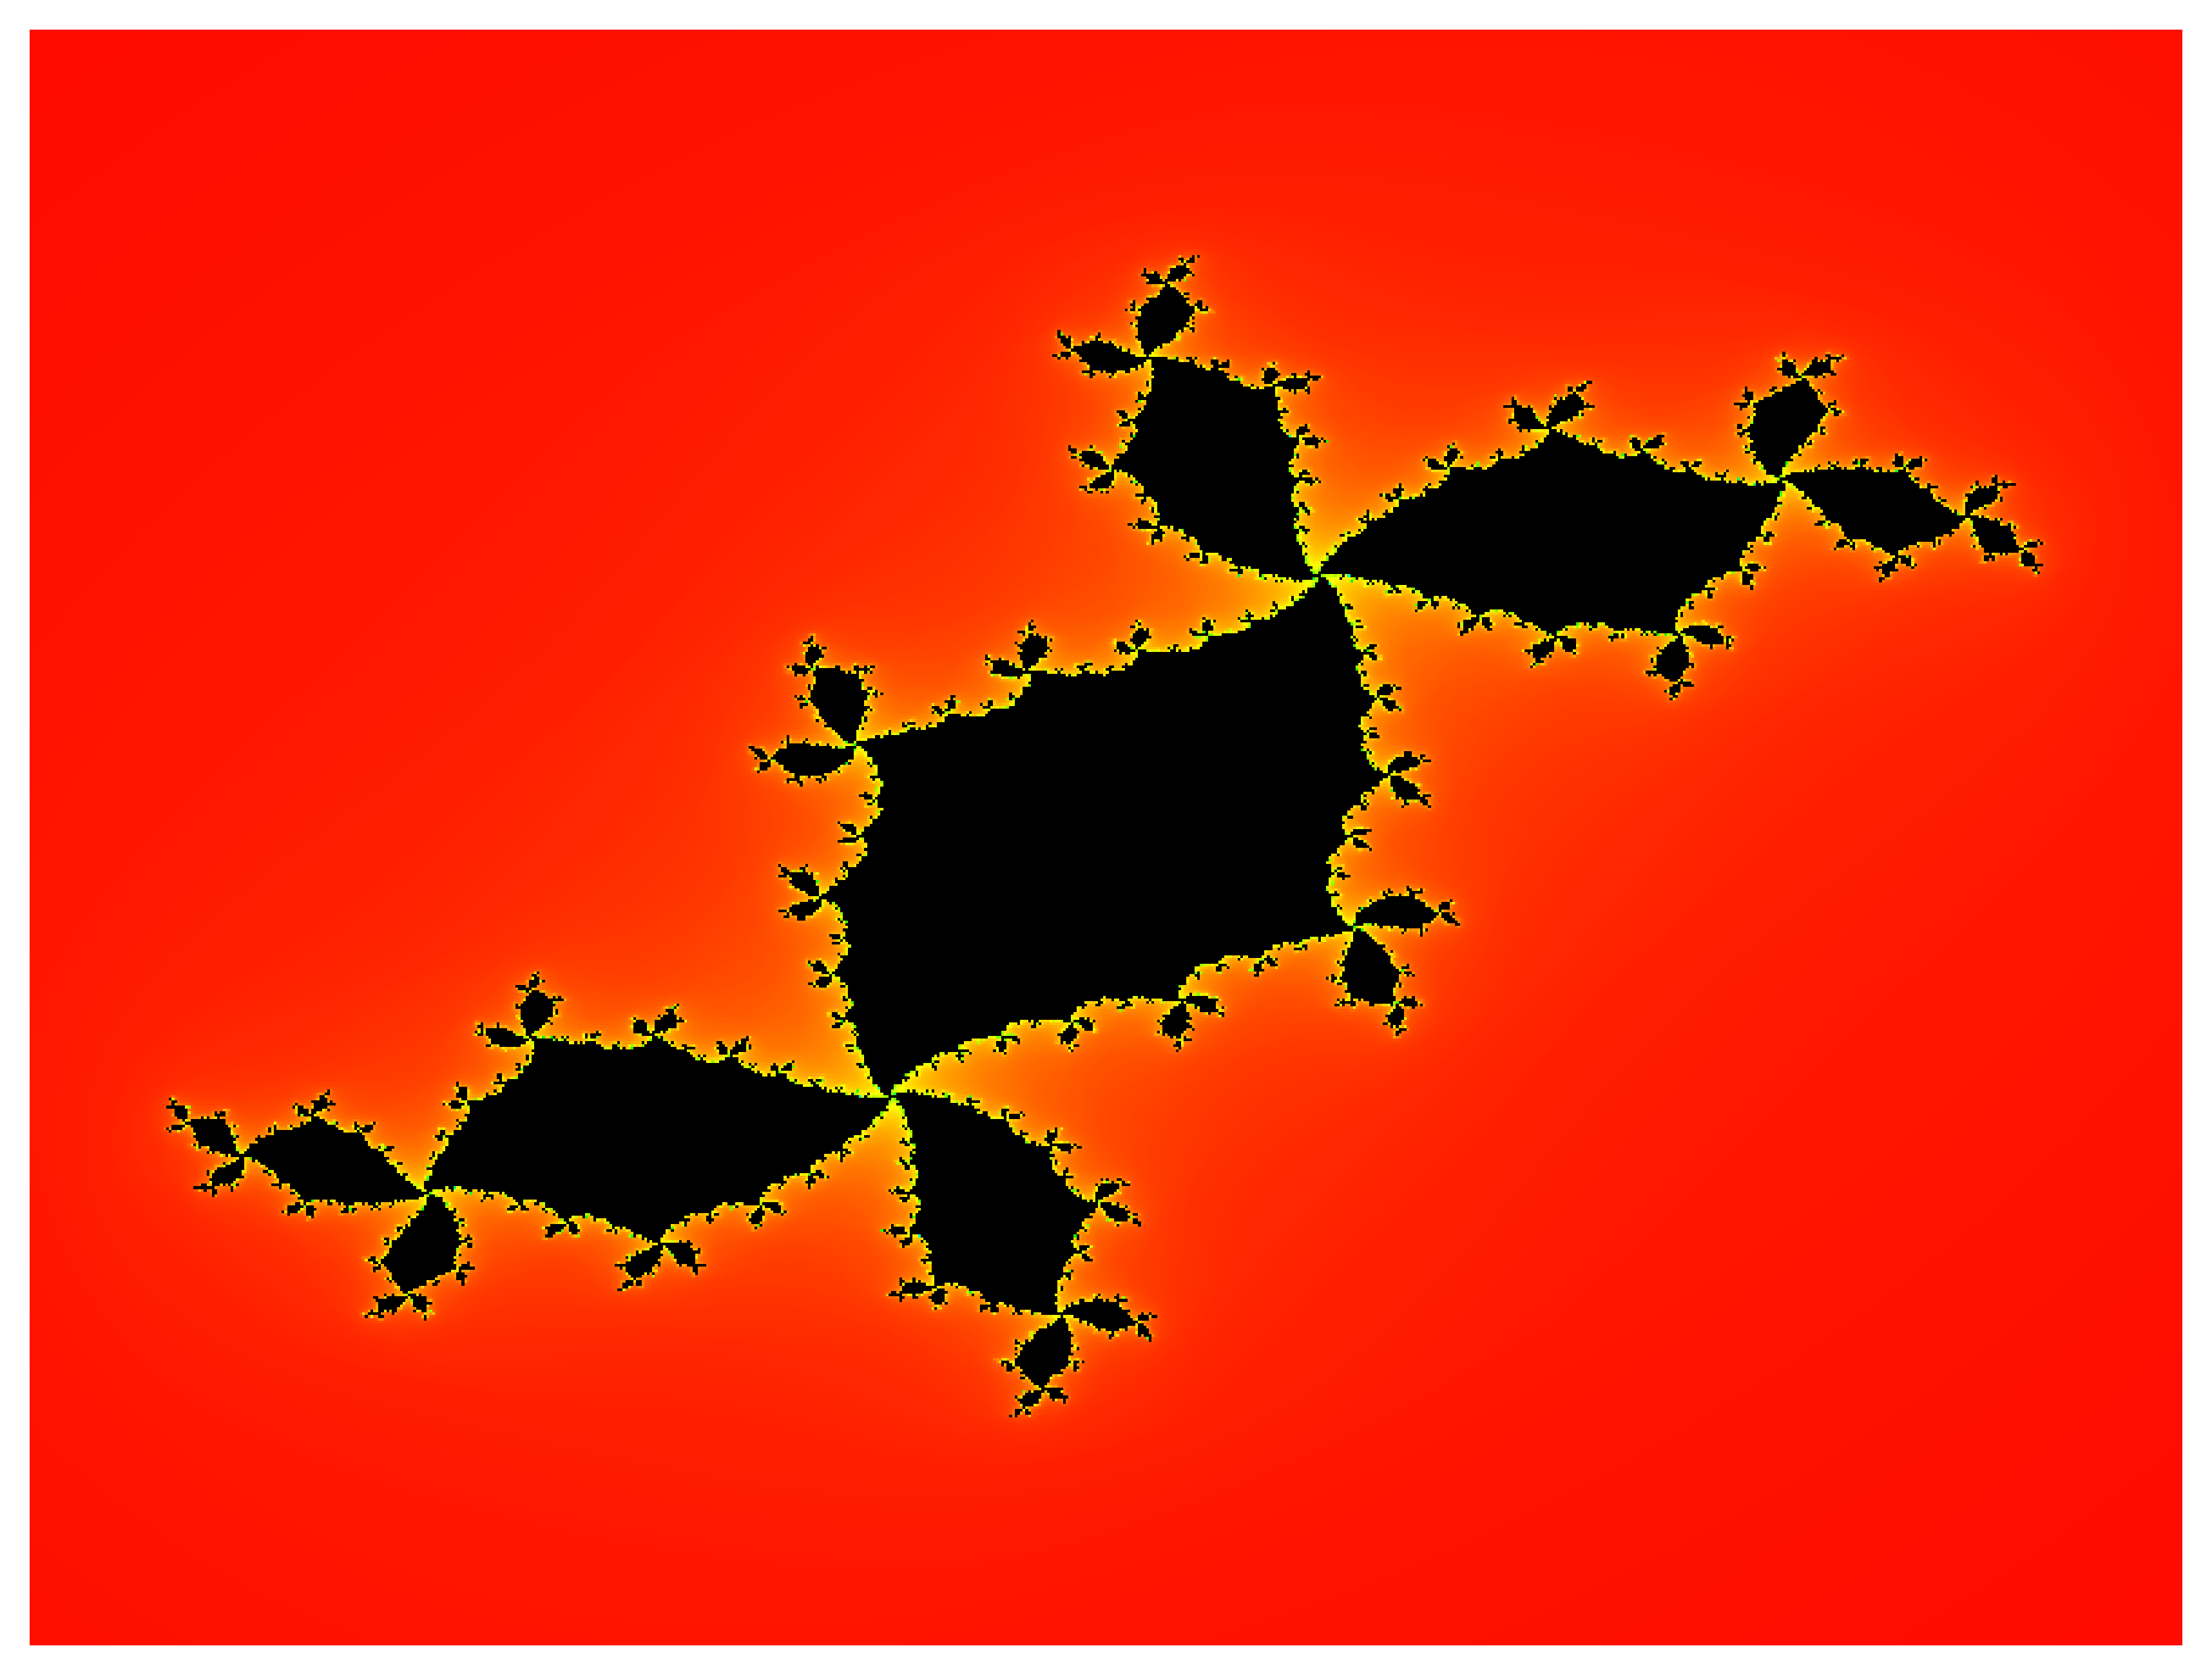
\includegraphics[width=\textwidth]{julia-set-1-colored.png}
%     \caption{$\filledinjulia(f)$ pro $f(z)=z^2 + 0{,}7885\cdot e^{\imag\cdot9\pi/16}$}
%     \label{fig:vyplnena-juliova-mnozina-1-obarveno}
% \end{figure}
% \begin{figure}[H]
%     \centering
%     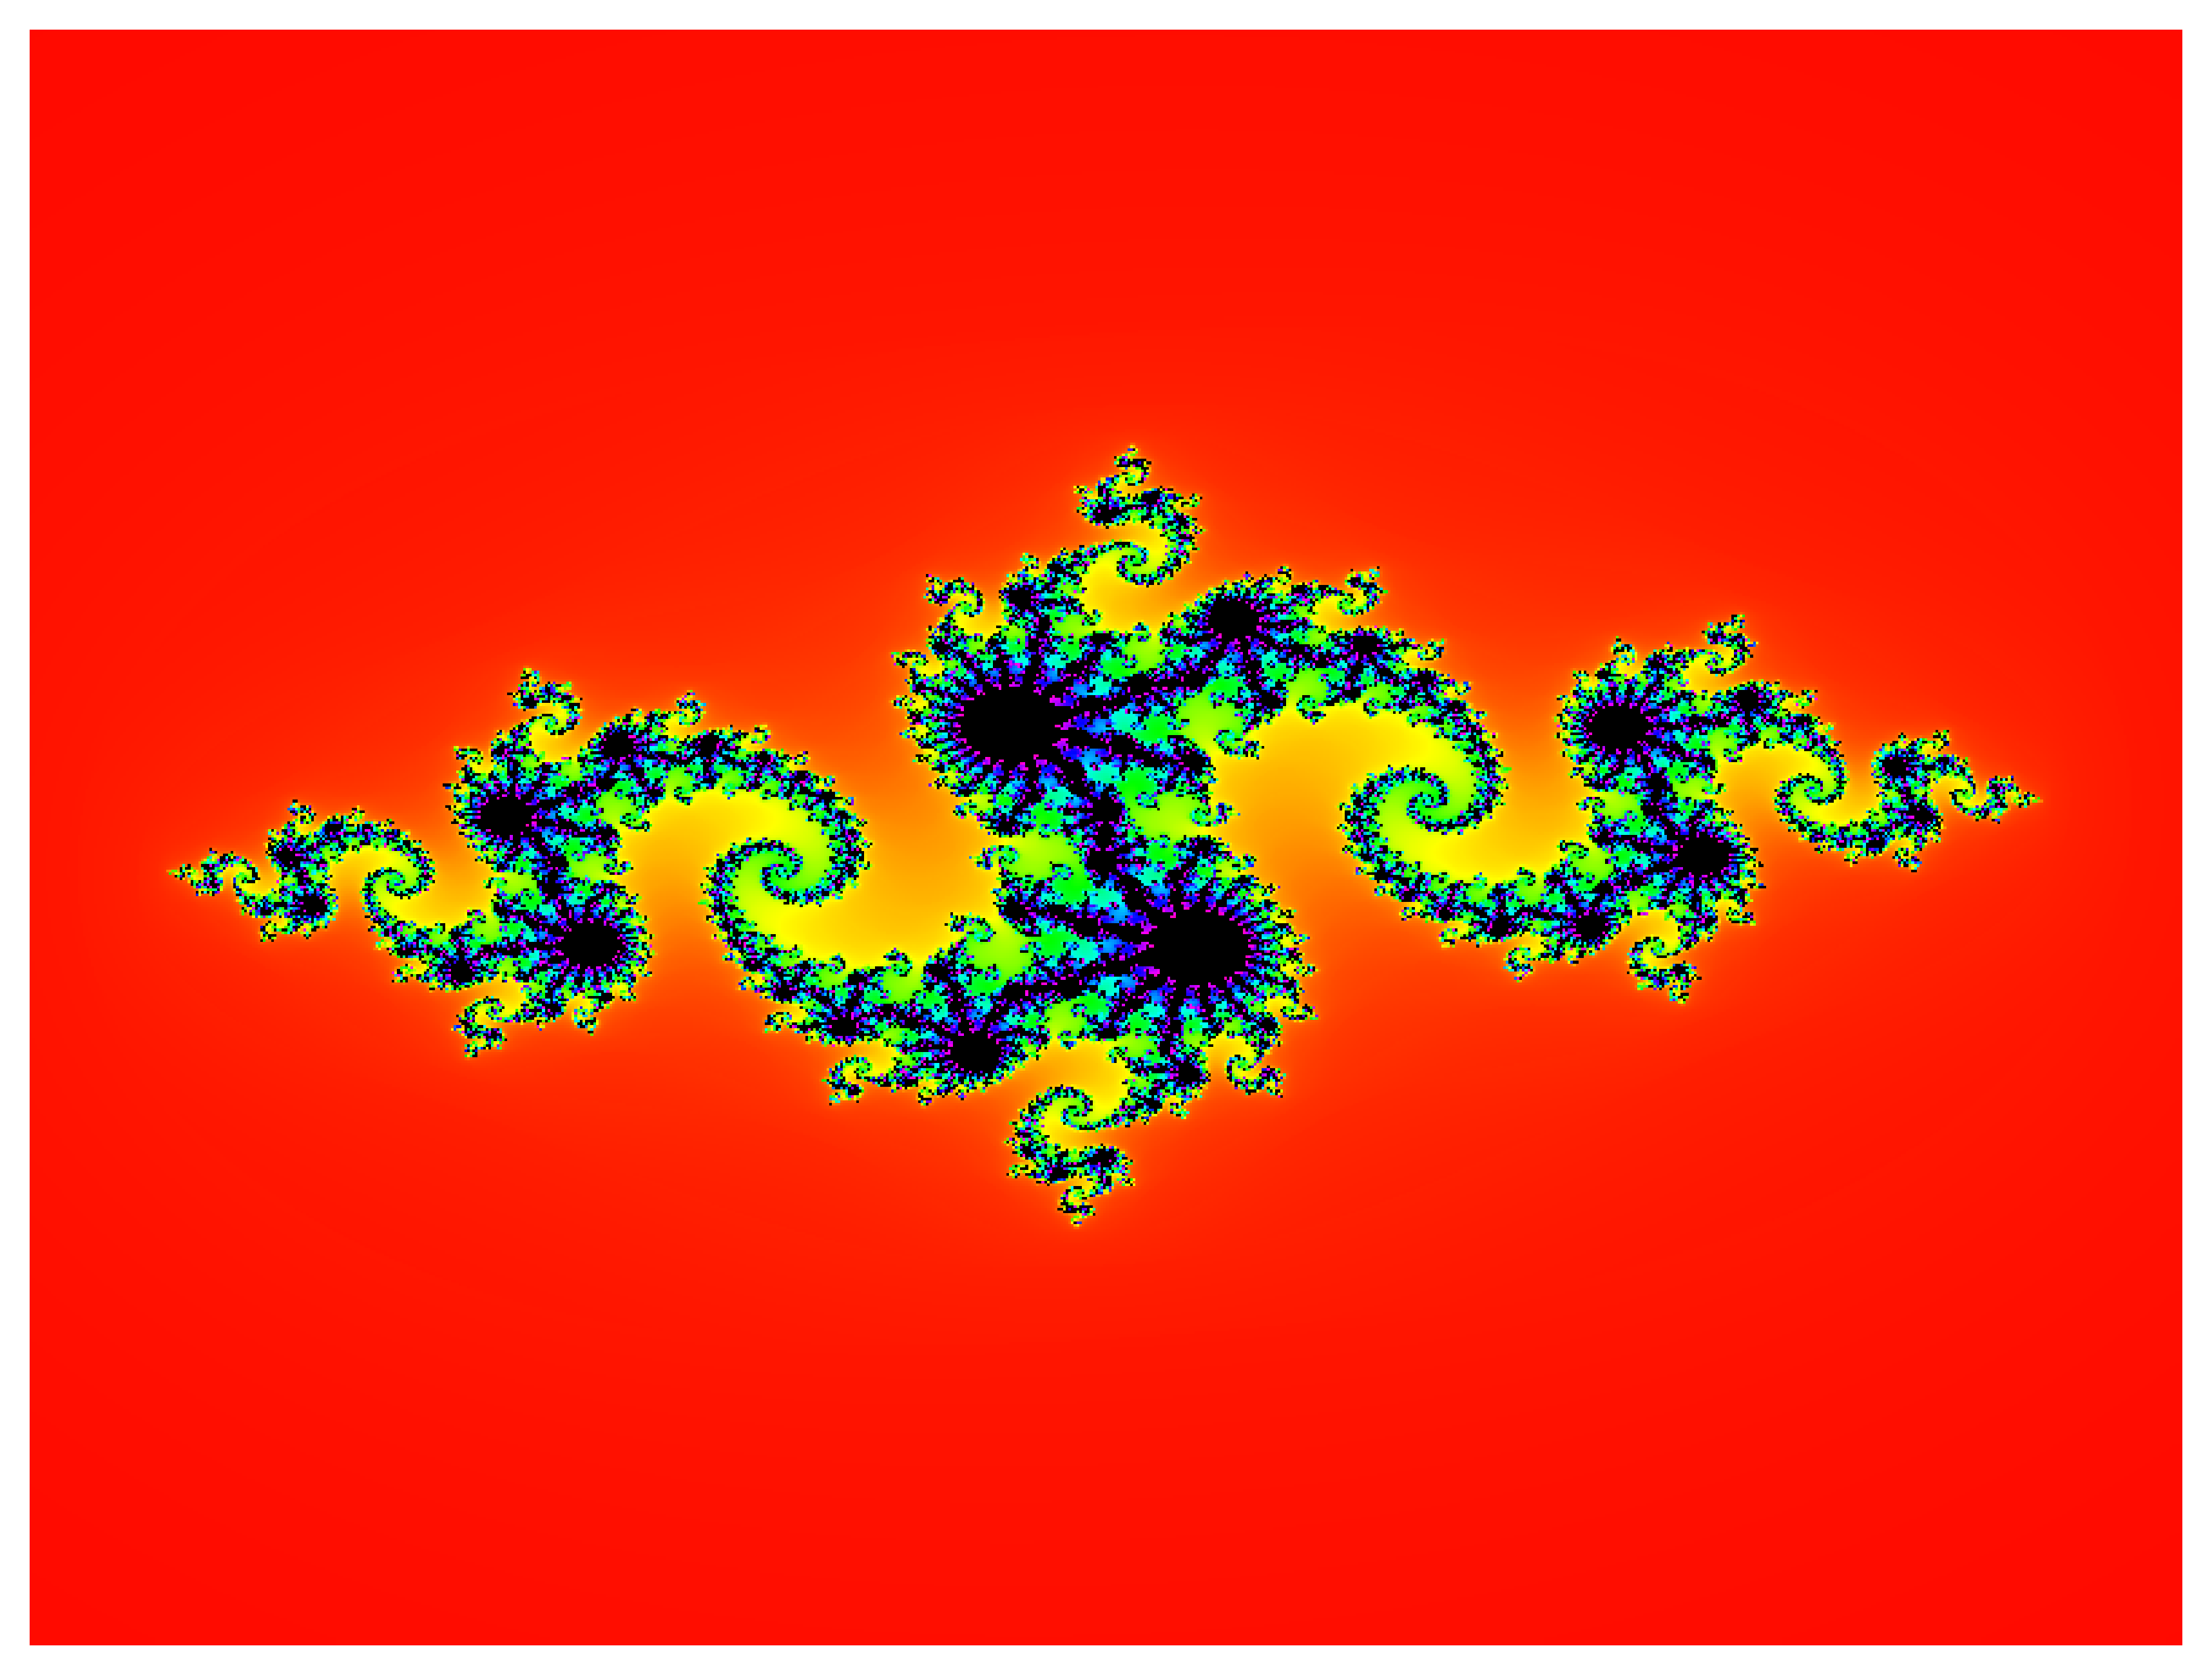
\includegraphics[width=\textwidth]{julia-set-2-colored.png}
%     \caption{$\filledinjulia(f)$ pro $f(z)=z^2 - 0{,}8 + 0{,}156\imag$}
%     \label{fig:vyplnena-juliova-mnozina-2-obarveno}
% \end{figure}

Barvu jednotlivým bodům $z\in\C$ přidělujeme podle toho, kolik iterací $k$ dané polynomiální funkce $f$ proběhlo, než hodnota $|f^{\circ k}(z)|$ překročila zadanou mez $r$ (viz lemma \ref{lem:test-konvergence-komplexniho-polynomu}). Vždy volíme pevný počet iterací funkce $f$, který aplikujeme na každý bod $\C$ (resp. na nějakou její podmnožinu). Podle zvoleného počtu se pak bude odvíjet i přesnost naší aproximace, avšak je třeba zvážit i výpočetní náročnost, která (celkem očekávatelně) roste se zvyšujícím se počtem iterací. Tomuto tématu (a mnohým dalším) se budeme věnovat v kapitole \ref{chapter:generovani-fraktalu}.
 
\subsection{Mandelbrotova množina}\label{subsec:mandebrotova-mnozina}

Mandebrotova množina patří patrně k jednomu z nejznáměnších fraktálů a stala se terčem nemalého množství publikací a popularizačních materiálů. Její mimořádně složitě vypadající vzhled a charakter přitom popisuje až překvapivě jednoduché pravidlo. Nejdříve si zavedeme následující funkci:
\[f_c(z)=z^2+c,\]
kde $c\in\C$. Tento konkrétní tvar polynominální funkce jsme již viděli v minulé podsekci, kde jsme se zabývali tzv. \emph{Juliovými množinami}\index{Juliova množina}\index{množina!Juliova}. Ty tvořily hranici množiny všech $z\in\C$, takových, že posloupnost $\set{f^{\circ k}(z)}_{k=1}^\infty$ je omezená. Ani zde se od původní myšlenky nevzdálíme, avšak budeme nyní zkoumat proměnnou $c$.
\begin{definition}[Mandelbrotova množina]\label{def:mandebrotova-mnozina}
    \emph{Mandebrotovu množinu}\index{Mandebrotova množina}\index{množina!Mandelbrotova} definujeme jako
    \[\mathfrak{M}=\set{c\in\C\mid \set{f_c^{\circ k}(0)}_{k=1}^\infty\notto\infty}.\]
\end{definition}
Upozorněme explicitně na fakt, že iterace vždy začínají pevně v bodě $z=0$. Mandebrotova množina je ve své podstatě konkrétní případ vyplněné Juliovy množiny. Stačí uvažovat funkci $g$ definovanou jako $g(c)=f_c(0)$. Pak zjevně $\mathfrak{M}=\filledinjulia(g)$ (viz obrázky \ref{fig:znazorneni-mandebrotovy-mnoziny} a \ref{fig:znazorneni-mandebrotovy-mnoziny-vybarveno}). Lze se však setkat i s jinými ekvivalentními definicemi. Např. $\mathfrak{M}$ lze charakterizovat i takto:
\[\mathfrak{M}=\set{c\in\C\mid\julia(f_c)\;\text{je souvislá}}.\]
Důkaz je opět delší, takže se znovu odkážeme na knihu \citep[str. 245]{Falconer1989}.
\begin{figure}[h]
    \centering
    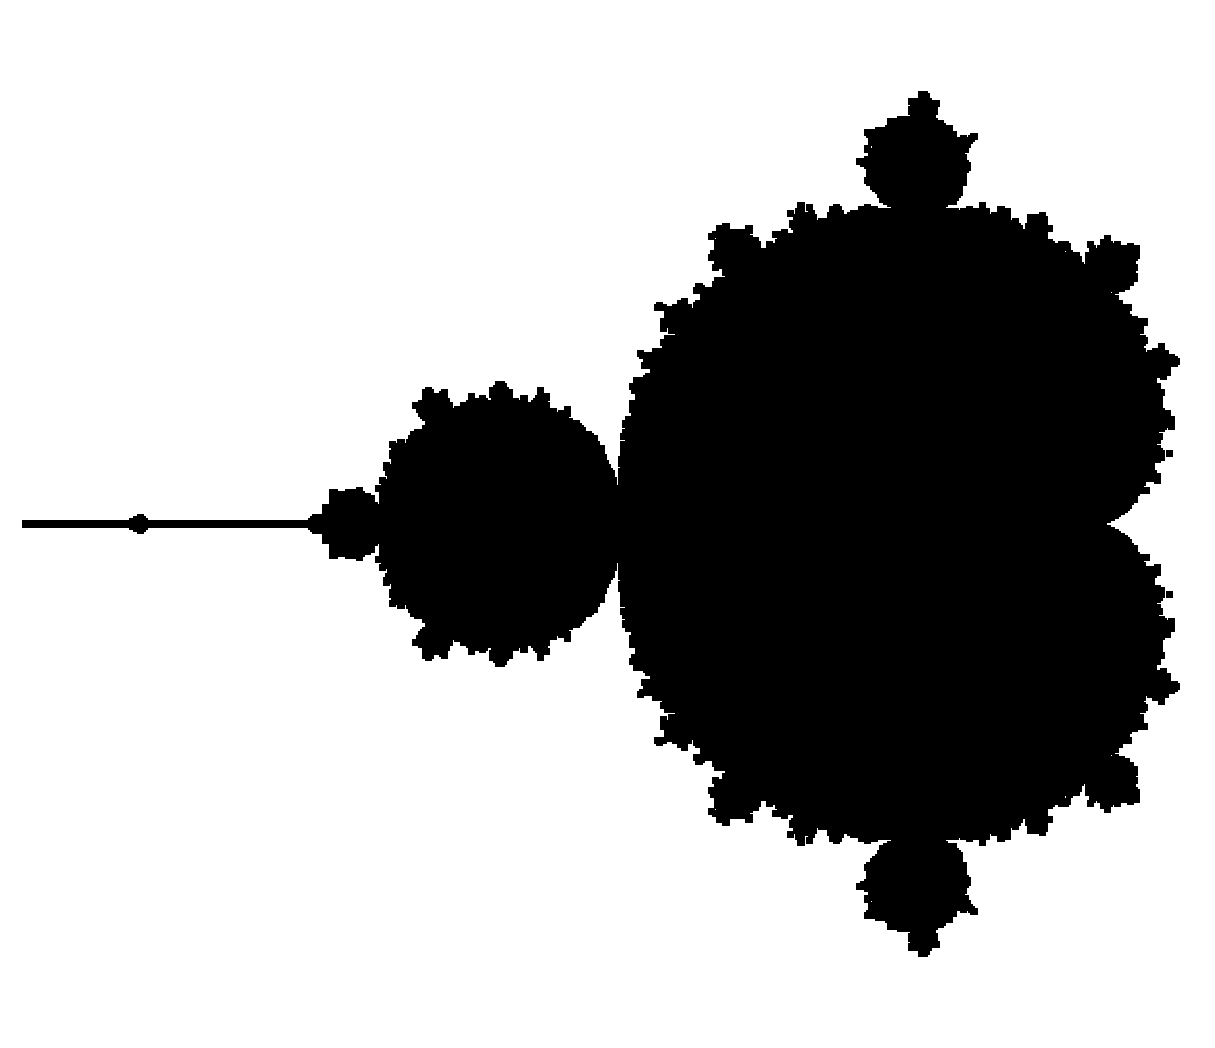
\includegraphics[width=\textwidth]{mandelbrot-set.pdf}
    \caption{Znázornění aproximace množiny $\mathfrak{M}$.}
    \label{fig:znazorneni-mandebrotovy-mnoziny}
\end{figure}
\begin{figure}[h]
    \centering
    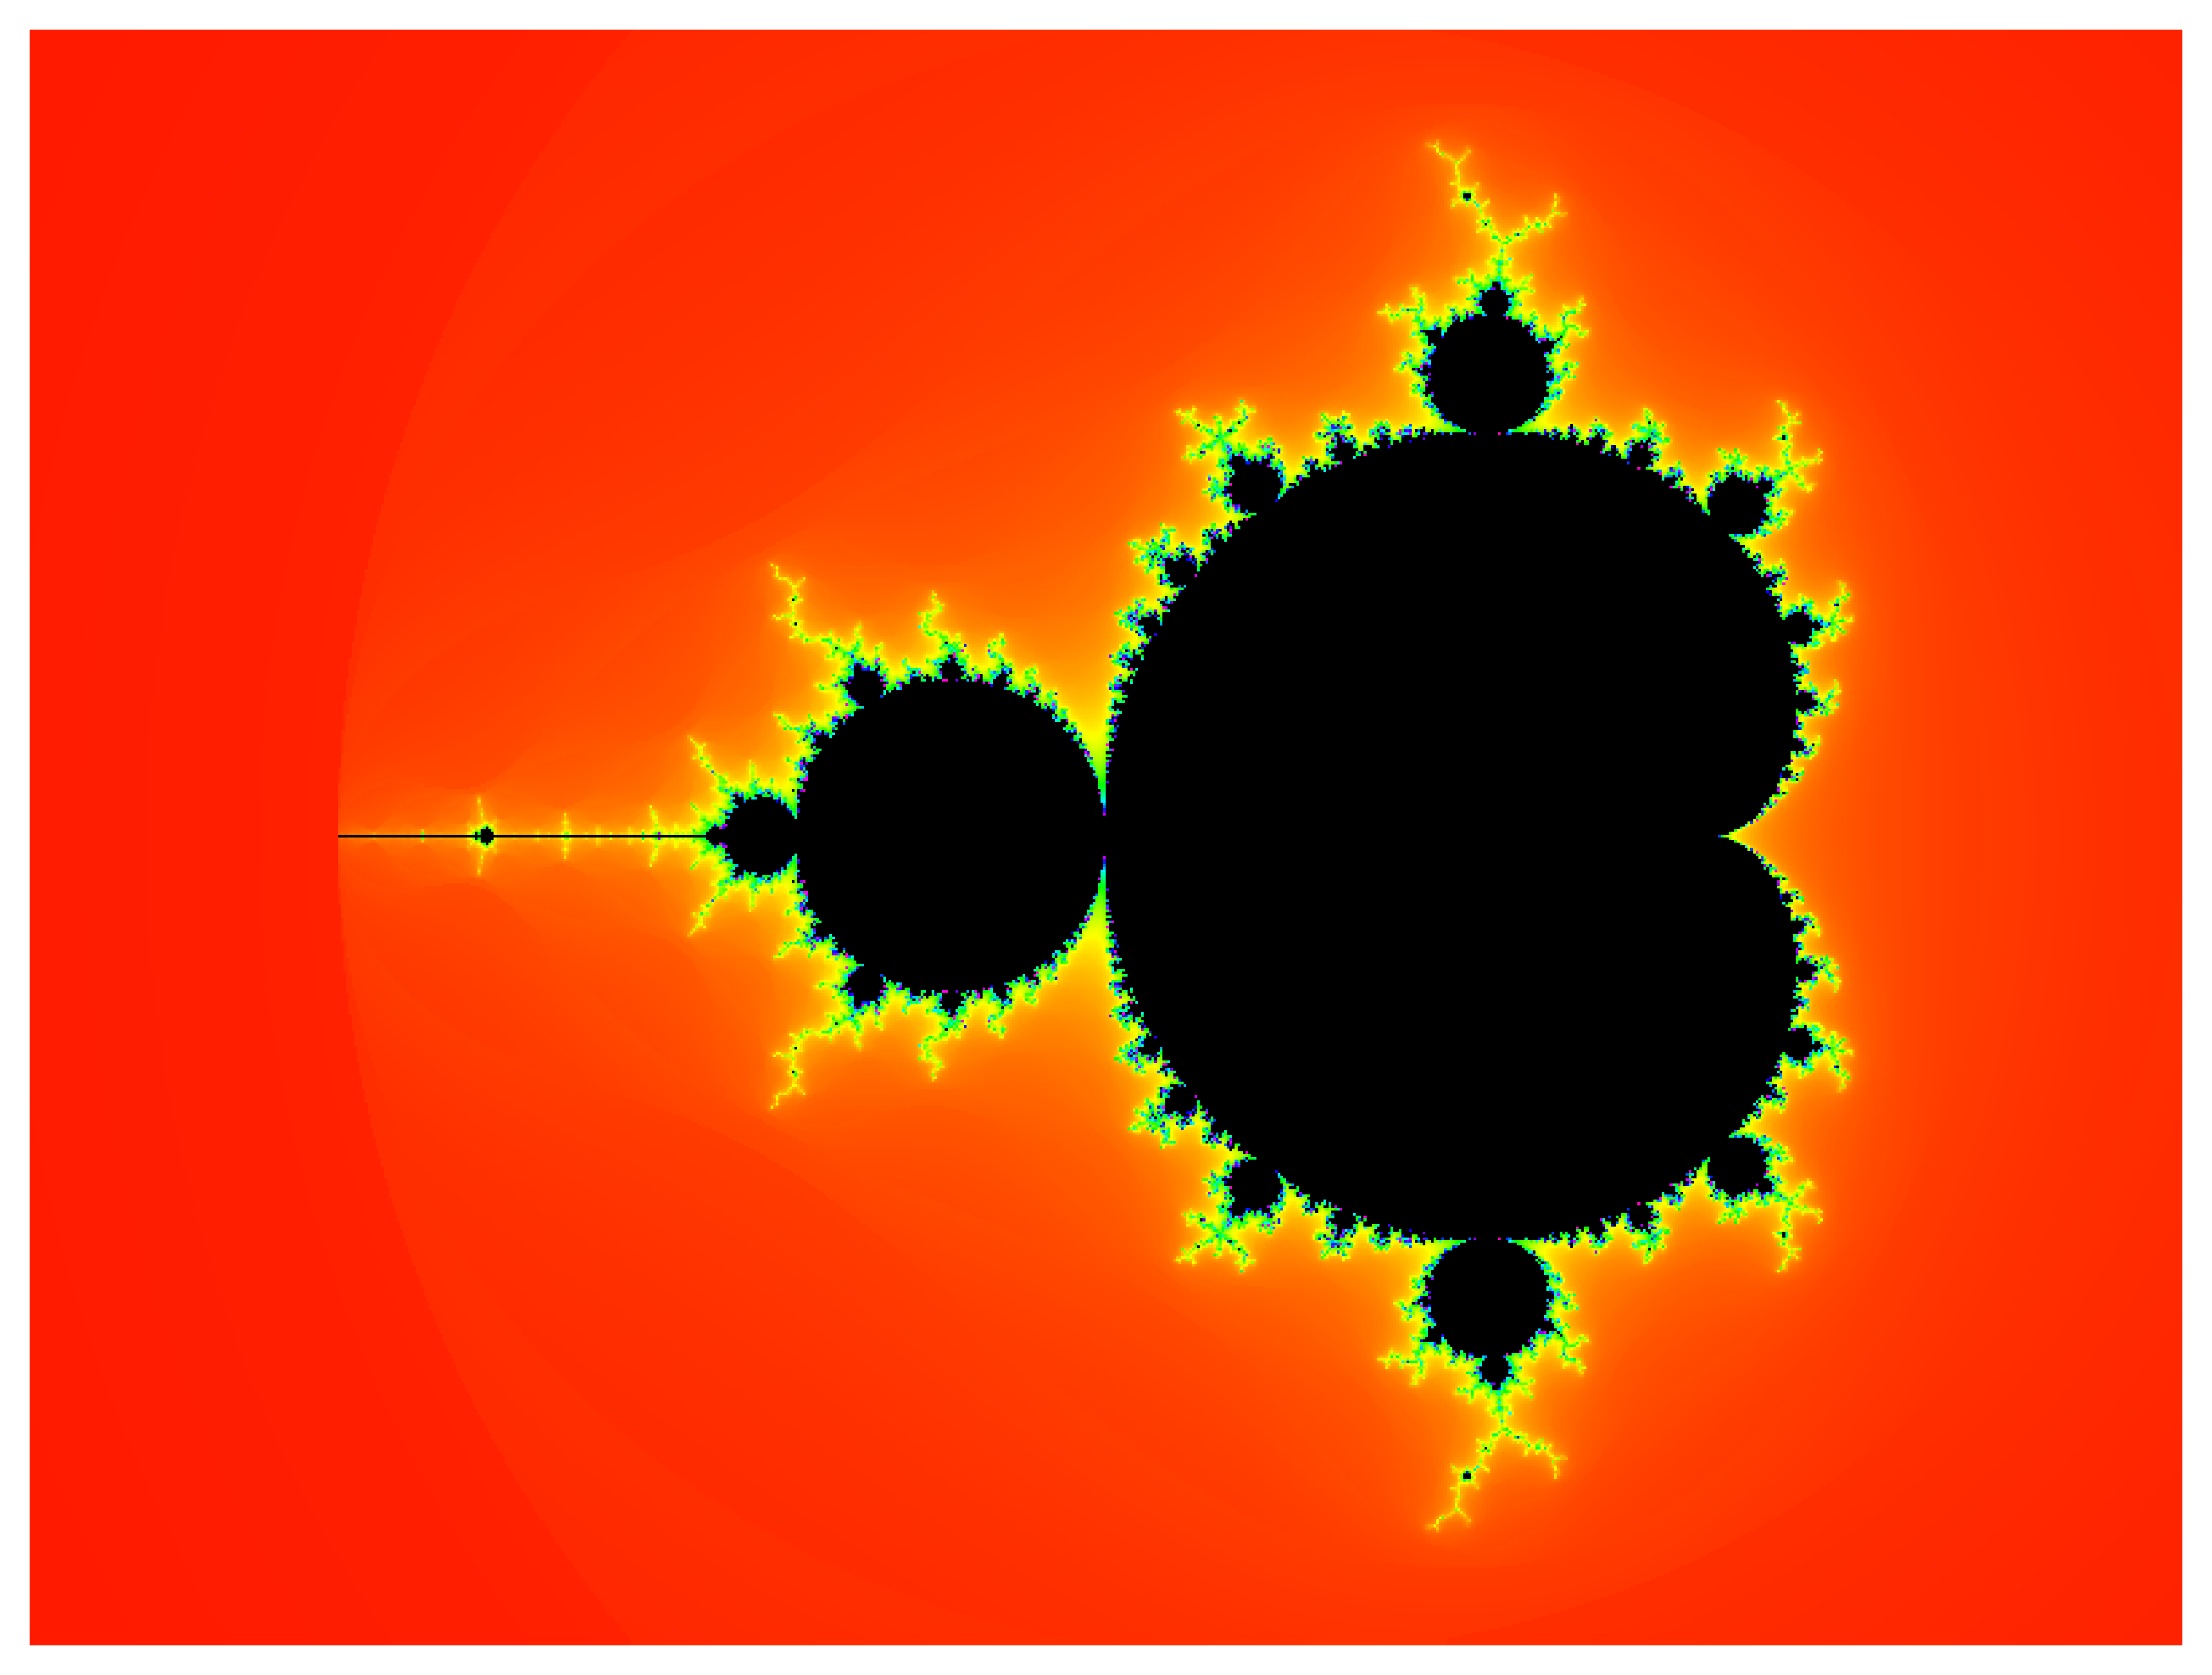
\includegraphics[width=\textwidth]{mandelbrot-set-colored.pdf}
    \caption{Barevné znázornění aproximace množiny $\mathfrak{M}$.}
    \label{fig:znazorneni-mandebrotovy-mnoziny-vybarveno}
\end{figure}
Jak je to s dimenzí? Tu lze odhadnout velice snadno. Zjevně platí, že $\dimH{\mathfrak{M}}\leqslant 2$. Zároveň však platí i druhá nerovnost $\dimH{\mathfrak{M}}\geqslant 2$, neboť $\mathfrak{M}$ obsahuje jako podmnožinu kouli $B_r(0)$, jejíž Hausdorffova dimenze je $2$. To zároveň silně podtrhuje naše konstatování neexistence jednotné definice termínu "fraktál", což jsme krátce rozebírali v sekci \ref{sec:co-je-to-fraktal}. Některé definice říkají, že za fraktální útvar považujeme soběpodobný útvar, jehož Hausdorffova dimenze je neceločíselná, avšak zde vidíme, že v tom případě bychom Mandebrotovu množinu nemohli považovat za fraktál.